% -----------------------------------------------------------------------------
\section{Introduction}
% -----------------------------------------------------------------------------

This paper aims to tackle memory-related performance issues, which represent one of the most crucial performance optimization topics. In hardware, memory access is optimized by providing faster memories closer to the chip (like HBM2), multi-level caches and transfer buffers, and even specialized explicit near-core memories (such as AVX512 registers or shared memory in Nvidia GPUs). Software developers benefit from these features by creating specialized, cache-aware algorithms, often tailored for a particular architecture.

The design of the way that the program data is laid out in memory is one of the crucial steps that ensures memory access performance. Even simple design choices like row- or column-major matrix storage impact the performance within the complex memory cache models by simplifying address translations, improving cache hit ratio and prefetching, or ensuring the alignment required for coalesced SIMD operations~\cite{clauss2000automatic,panda2001cache}. For parallel algorithms, the complexity of the problem becomes much broader because of cache-line collisions, false-sharing, non-uniform memory architectures, a variety of synchronization issues~\cite{bethel2015improving,heinecke2008parallel,weidendorfer2007latencies}, and other factors. Many-core platforms (GPUs in particular) only amplify this by enforcing specific data access patterns in lockstep execution, advocating the use of programmer-managed caches (like shared memory), and having a significantly lower cache-to-core ratio in comparison to the CPUs~\cite{guide2013cuda}.

The best layout is quite often elusive and needs to be discovered empirically. Furthermore, it often differs even among the utilized cache levels~\cite{weber2017matog,hawick2011hypercubic,krulivs2020detailed}. Consequently, the optimal implementations are often complicated, and most of the optimization-relevant code is not portable between hardware architectures. Enabling simple implementations of layout-flexible data structures and algorithms would improve the code portability (and value); however, systematic approaches are quite rare, often over-complicating the code logic and making the algorithm implementation not maintainable or usable beyond the community of specialists.


\subsection{Motivational example}

To explain the motivation, objectives, and contributions of our research, we have selected a matrix multiplication problem widely known in computer science. For the sake of simplicity, we use the most straightforward implementation with $\mathcal{O}(N^3)$ complexity (computing $C = A \times B$ of square matrices $N^2$):

\begin{minted}[fontsize=\scriptsize]{c++}
    for (size_t i = 0; i < N; ++i)
        for (size_t j = 0; j < N; ++j) {
            C[i][j] = 0;
            for (size_t k = 0; k < N; ++k)
                C[i][j] += A[i][k] * B[k][j];
        }
\end{minted}

Having a fixed algorithm structure (i.e., order of the operations), the memory layout of the matrices is the main issue affecting the performance. In this context, the layout is defined by transforming the abstract indices ($i,j$) into an offset, subsequently used to compute the actual memory address. For instance, the most common matrix layout is row-major, which computes the offset as $i*W + j$ (where $W$ is the width of the matrix). A few examples of possible layouts are depicted in Figure~\ref{fig:layout}.

\begin{figure}
    \begin{subfigure}{.19\textwidth}
        \centering
        \includegraphics[width=.9\linewidth]{noarr/figures/matrix-row-major}
        \caption{row-major}
        \label{fig:layout-row}
    \end{subfigure} 
    \begin{subfigure}{.19\textwidth}
        \centering
        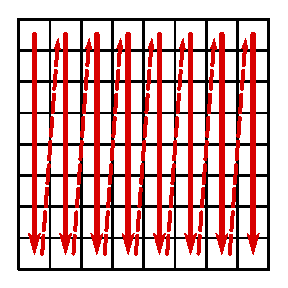
\includegraphics[width=.9\linewidth]{noarr/figures/matrix-col-major}
        \caption{col-major}
        \label{fig:layout-col}
    \end{subfigure}
    \begin{subfigure}{.19\textwidth}
        \centering
        \includegraphics[width=.9\linewidth]{noarr/figures/matrix-tiled}
        \caption{row-tiles}
        \label{fig:layout-tile}
    \end{subfigure}
    \begin{subfigure}{.19\textwidth}
        \centering
        \includegraphics[width=.9\linewidth]{noarr/figures/matrix-zcurve}
        \caption{z-curve}
        \label{fig:layout-zcurve}
    \end{subfigure}
    \begin{subfigure}{.19\textwidth}
        \centering
        \includegraphics[width=.9\linewidth]{noarr/figures/matrix-hcurve}
        \caption{Hilbert curve}
        \label{fig:layout-hcurve}
    \end{subfigure}
    
    \caption{Examples of common matrix layouts}
    \label{fig:layout}
    \vspace{-10pt}
\end{figure}

The aforementioned code sample used traditional C notation \mintinline{c++}{A[i][j]} which enforces the row-major layout, which is sub-optimal for this algorithm. Having the second matrix in a col-major layout or using a z-curve for all matrices will improve cache utilization, and the algorithm would run several times to several orders of magnitude faster, depending on the platform. Therefore, we need to introduce layout flexibility into the code.

A typical object-oriented solution would be to create a class abstraction that would define a uniform interface for accessing matrix elements whilst enabling different implementations through derived classes. A slightly better and more reusable solution would be to separate the offset computation into a policy class that would be injected into the matrix as a template parameter:

\begin{minted}[fontsize=\scriptsize]{c++}
    class RowMajor {
        static size_t offset(size_t i, size_t j, size_t W, size_t H) {
            return i*W + j;  
        }
    };

    template<typename T = float, class Layout = RowMajor>
    class Matrix {
        /* ... */
        T& at(size_t i, size_t j) {
            return _data[Layout::offset(i, j, _W, _H)];
        }
    };
\end{minted}
  
The policy class makes the matrix implementation flexible (in terms of selecting the proper layout) and efficient (since the compiler can inline the static method). However, several drawbacks make this solution imperfect. The interface between the \texttt{Matrix} class and its layout policy (\texttt{RowMajor}) is created ad-hoc by the author of the main class, which complicates the code reusability of the layout policies in potentially compatible situations. The interface also prevents efficient constant propagation and caching of intermediate values. Furthermore, the strong encapsulation may prevent low-level optimizations, portability to other architectures (e.g., GPUs), and complicate data structure composition (e.g., when matrices in an array need to be interleaved).

We aim to design a more straightforward, more programmer-friendly solution to implementing \emph{layout-agnostic} algorithms, focusing on enabling performance optimizations and parallel processing.


\subsection{Objectives and contributions}

Our main objective was to create a library that allows the users to quickly adapt their algorithms and data structures for different memory layouts, with a~particular focus on the following targets:

\begin{itemize}
    \item Once an algorithm is adapted, it becomes layout-agnostic --- i.e., no subsequent internal code modifications should be required to change the layout of the underlying data structures.
    \item The layout representation should not be coupled with memory allocation so that it could be used in different scenarios and different memory spaces (i.e., directly applicable with memory-mapped files or GPU unified memory).
    \item The interface should define an easily comprehensible abstraction for \emph{indexing} (offset computation) that would hide its (possibly complex) nuances.
    \item The indexing mechanism should enable the compiler to evaluate constant expressions at compile time (e.g., fold constant dimensions of a structure into the generated code).
    \item The code overhead should be minimal, preferably smaller than with well-established practices, such as providing template policy classes to govern layout or allocation.
\end{itemize}

We have implemented \Noarr{} header-only library\footnote{\Noarr{} is available as open-source on GitHub under MIT license: \url{https://github.com/ParaCoToUl/noarr-structures}} for C++ as a prototype that achieves the outlined objectives. C++ was chosen as a widely-used mainstream language that provides complete control over memory layout and allocation and is widely used for programming performance-critical applications, including parallel HPC systems and GPGPU computing. Its fundamental features, like the templating system and operator overloading, open possibilities for generic programming, compile-time optimizations, and the design of a functional-like interface, which simplifies the use of the library. Furthermore, the separation of indexing from (CPU-specific) memory management allowed us to directly utilize the library with Nvidia CUDA code, easily porting the layout-agnostic code on contemporary GPUs.

We believe that \Noarr{} will make a significant contribution to simplifying the coding process and increasing performance in many scenarios, especially:
\begin{itemize}
    \item Empirical exploration of possible layouts --- i.e., finding the optimal combination of layouts for given data structures and algorithms by measuring the performance of all possible implementations.
    \item Implementing applications and libraries in which the optimal layout of data structures needs to be selected at runtime (e.g., based on the size of the problem or the best available architecture).
    \item Allowing simple yet efficient (semi)automatic layout transformations in case the input or output layouts differ from the optimal layouts for the computation.
\end{itemize}

Although the issues mentioned above can be identified in a large variety of data structures and algorithms, we are focusing mainly on regular data structures such as nested multi-dimensional arrays and structures (in the C/C++ sense). However, despite this narrow scope, we have identified that this problem is quite challenging, especially regarding optimizations for massively parallel environments like GPUs.

% Furthermore, \Noarr{} library enables research of semi-automated or automated selection of the best memory layout for given problem configuration, and automatic layout transformations of data structures that are often required when moving the data between memory types (e.g., when a row-major matrix from disk is transferred to a column-major format in memory). Here, we mainly demonstrate the possibility of automating the layout transformation process. Although the automated selection of the best data layouts for algorithms is easy to implement with the current version of \Noarr{}, a rigorous review of the methodology is well beyond the scope of this paper.


The paper is organized as follows. Section~\ref{sec:layouts} explains the key principles and benefits of the layout-agnostic algorithm design. The performance aspects of offset computation overhead are summarized in Section~\ref{sec:perf}. In Section~\ref{sec:implementation}, we provide insights into the current implementation of the \Noarr{} library. Related work and main conclusions are summarized in Sections~\ref{sec:relwork} and \ref{sec:conclusion}.
